\label{objectifs}
Le phénomène physique à traiter dans le cadre de cette activité expérimentale de physique était la « conduction ». 
Nous étions le premier groupe à travailler sur ce sujet et démarrions de rien. 
Aussi, nous avons choisi de nous intéresser à la mesure de conductivité \textit{électrique}.

La \textbf{conductivité électrique} représente la capacité d'un corps à conduire le \textit{courant électrique} ; 
ce qu'on entend par « courant électrique », c'est un déplacement de charges électriques 
(ces charges pouvant être négatives ou même positives, nous y reviendrons).

\bigskip
Le fil conducteur de notre démarche fut l'idée d'AE à proposer aux élèves de première année, 
idée qui se base sur le constat suivant :
\textbf{On peut caractériser incontestablement un semiconducteur (SC) en effectuant 
une mesure de conductivité en fonction de la température.}
Par caractériser on entend déterminer s'il s'agit d'un SC pur, dopé voire dégénéré (voir Figure \ref{conduc}).

\begin{figure}
  \centering
  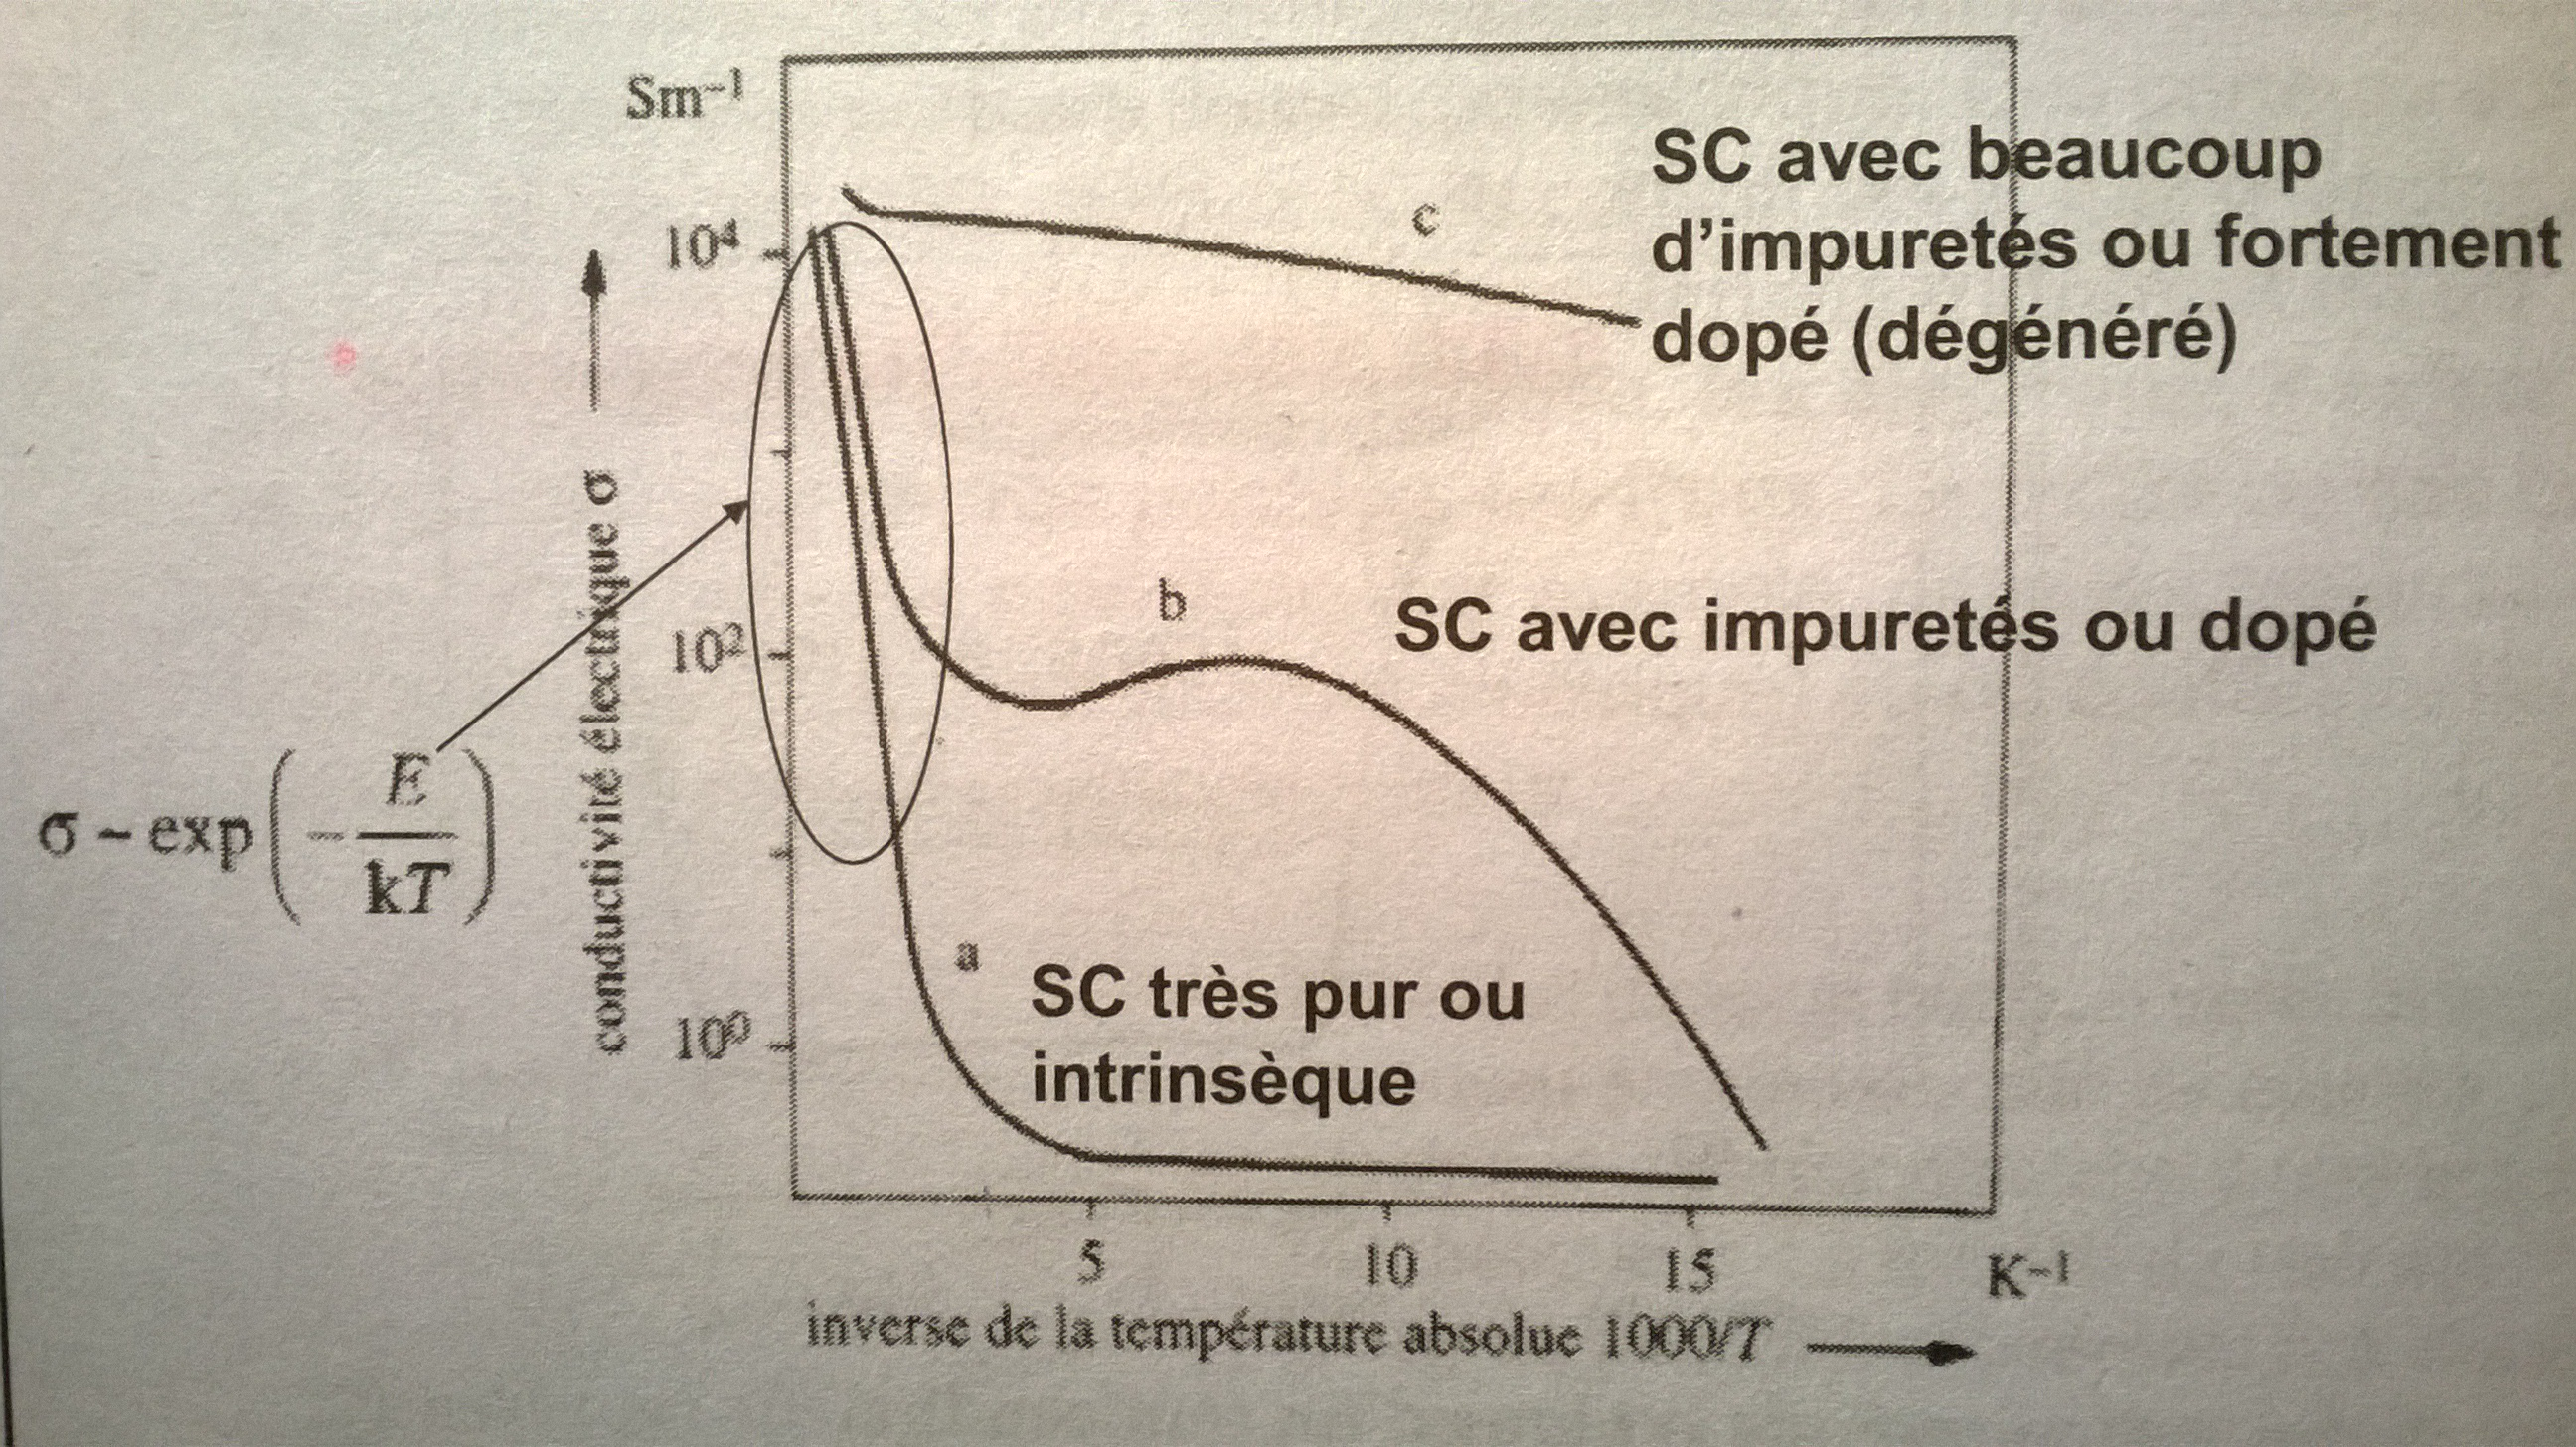
\includegraphics[width=12cm]{./images/conductivite.jpg}
  \caption{Les courbes ci-dessus illustrent le fait
  qu'une étude de conductivité en fonction de la température appliquée à un échantillon de matériau SC
  permet d'identifier s'il s'agit d'un SC pur, dopé ou dégénéré.}
  \label{conduc}
\end{figure}

\bigskip
L'idée d'AE est la suivante :
Mettre à la disposition des élèves de première année 2 types de SC, un pur et un dopé. 
Le premier objectif est de déterminer qui est qui (lequel est dopé et lequel est pur), 
en réalisant une étude de la conductivité de chaque échantillon 
en fonction de la température.

Une remarque à ce stade : cette étude de conductivité ne permet pas de dire si le SC dopé est de type N ou P.

Le second objectif est alors de déterminer si le SC dopé identifié grâce à l'étude de 
conductivité est de type N ou P.
Comment ? En réalisant une mesure de la tension Hall de l'échantillon.
En effet, la tension Hall étant reliée notamment au signe des porteurs de charge, si l'on mesure une tension négative, 
on mettra alors bien en évidence des électrons, et donc on déduira qu'il s'agit d'un dopé N.
Si par contre on mesure une tension positive, on mettra alors en évidence des porteurs de charges positive, les trous !
Il s'agira alors d'un dopé P.

Seule la première mesure a pu être effectuée, le montage Hall n'a malheureusement pas pu être testé.

\bigskip
Nos objectifs étaient donc de mettre en place les deux montages correspondant à ces manipulations, 
et de réaliser effectivement les mesures suivantes :
\begin{enumerate}
\item mesure de conductivité en fonction de la température ;
\item mesure de la tension Hall d'un échantillon.
\end{enumerate}
Enfin, nous voulions piloter et acquérir les mesures sur ordinateur via l'environnement 
de développement graphique \textit{LabVIEW}.
